\chapter{Problem}
Et pendul skal styres til at stå lodret på en bevægende platform.
\begin{figure}[htbp]
        \centering
        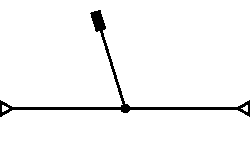
\includegraphics[width=0.95\textwidth]{pendul.png}
        \caption{Pendul på sin ``slæde''}
        \label{fig:label}
\end{figure}
Modellen for dette system er:
\begin{equation}
        m\g l \g \Ddot{\theta} + m \g g \g sin(\theta) + k_f \g l \ \dot{\theta} = \frac{T}{l} + \delta_c(t)
\end{equation}

Konstanterne i dette system er dog ikke sikre, og de kan derfor antageforskellige værdier:
\begin{equation}
        \begin{split}
                0.095 \leq &m \leq 0.105 \\
                &l = 0.305 \\
                0.4 \leq &k_f \leq 0.6 \\
                &g = 9.81 \\
        \end{split}
\end{equation}

Forstyrelsen i form af slædens bevægelse kan estimeres til:
\begin{equation}
        \delta_c(t) = 0.0934 \g 5/2000 \g sin(t)
\end{equation}

Målsætningen er at lave en ``Sliding mode'' kontroller som kan få pendulet til at stå lodret $(\theta, \dot{\theta})= \pi, 0$. Fejlen på $\theta$ må maksimum være op til 0.1 radianer til en af siderne, og rotations hastigheden af pendulet ($\dot{\theta}$) må maks være 0.01

Den fundne kontroller skal først tested i suimulering, og skal derefter testes på en rigtig platform.